\documentclass{article}
\usepackage{graphicx}
\usepackage{listings}
\graphicspath{ {images/} }

 \pagenumbering{arabic}
 \usepackage{array}
 





\begin{document}


\includegraphics[width=10cm, height=5cm]{logo} \break \break

\centering {\textbf{Computer Science and Engineering} }\\

 \centering{A.A. 2016/2017} \\
\centering{Software Engineering 2 Project:} \\

\centering{\textbf{ Power\&Joy} }\break



\centering{\textbf{\large{Project Plan }} }\break \break

\centering{January 22, 20167}\break





\begin{flushright}


Prof. Luca Mottola\break 
Joshua Nicolay Ortiz Osorio \ Matr: 806568 \\
Michelangelo Medori \ Matr: 878025

\end{flushright}

\newpage

\centering {\textbf{Index}} \\    %INDEX
\begin{enumerate}

\item Introduction




\begin {enumerate}
\item [1.1] Revision History
\item [1.2] Purpose and Scope
\item [1.3] List of Definitions and Abbreviations 
\item [1.4] List of Reference Documents

\end{enumerate}

\item Project size, cost and effort estimation


\begin {enumerate}
\item [2.1] Size estimation: Function Points

\begin{enumerate}
\item[2.1.1]{Internal Logic Files(ILFs)}
\item[2.1.2]{External Logic Files(ELFs)}
\item[2.1.3]{External Inputes (EIs)}
\item[2.1.4]{External Inquiries(EQs)}
\item[2.1.5]{External Outputs(EOs)}
\item[2.1.6]{Overall Estimation}
\end{enumerate}
\item [2.2] Elements to be Integrated 
\begin{enumerate}
\item[2.2.1]{Scale Drivers}
\item[2.2.2]{Cost Drivers}
\item[2.2.3]{Effort Equation}
\item[2.2.4]{Schedule Estimation}

\end{enumerate}



\end {enumerate} 




\item[3] Schedule



\item[4] Resource Allocation



\item[5] Risk Management 



\item [6]ChangeLog
\item[7] Hours of Work


\end{enumerate}

\newpage   
\begin{flushleft}  

  \section{Introduction}	% 1)INTRODUCTION
  \subsection{Revision History} 	% 1.1)REVISION HISTORY
  
  \begin{center}
    \begin{tabular}{ | p{2cm} | p{2cm} |  p{7 cm} | p{4cm} |}
    \hline
    \textbf{Version} &  \textbf{Date} & \textbf{Author(s)} & \textbf{Summary}  \\ 
    \hline
    
    1.0 & 22/01/2017 & Joshua Nicolay Ortiz Osorio and Michelangelo Medori & initial release
     \\ 
  \hline

  
    \end{tabular}
\end{center}
\vspace{1cm}
\subsection{Purpose and Scope} %1.2
This is the Project Plan Document for the Power\&Joy car sharing management system. The aim of this document is to provide a detailed estimation of the size and the cost, given by an accurate analysis of the complexity of the functionalitires  of the system.
After the following list of definitions, acronyms and abbreviations and reference documents, in section 2 we are going provide first a size estimation using the Function Points approach (chapter 2.1 ) and a cost/effort estimation using the COCOMO model. 
In section 3 we are going to describe a possible schedule for the project development, which  covers all the activities involved in the development, ranging  from the requirements analysis to the implementation and testing activities.
In section 4 we are going to assign to each member of our development group various tasks in order to allocate the right resources to every task. 
Finally, section 5 contains an analysis of the risks that arise about the project development, and some overall conclusions.

\newpage
\subsection{List of Definitions, Acronyms, Abbreviations} %1.3
\subsubsection{Definitions} %1.3.1




\subsubsection{Acronyms} %1.3.2
\begin{itemize}

\item{ FP: Function Points}
\item{ILF: Internal Logic File}
\item{ELF: External Logic File}
\item{ EI: External Input}
\item{ EO: External Inquiry}
\item{ EQ: External Output}
\item{DBMS: Database Management System.}
\item{UI: User Interface.}
\item{GPS: Global Positioning System.}
\item{TDI : Total Degree of Influence}
\item{VAF: Value Adjustment Factor}
\item {UFP: Unadjusted Function Point}
\item{AFP : Adjusted Function Point}
\item{SLOC: Source Lines Df Code}
\


\end{itemize}



\subsubsection{Abbreviations} %1.3.3


\subsection{Reference Documents} %1.4
\begin{itemize}
\item{Assignment document.pdf}
\item{RASD (Requirement Analysis and Specification Document 4.0.pdf)}
\item{Project Plan Example Document.pdf}
\item{The Function Points complexity evaluation tables}
\item The COCOMO II Model Definition Manual (version 2.1, 1995 ? 2000
Center for Software Engineering, USC).

\end{itemize}

\newpage
\section{Project size, cost and effort estimation} %2
in this section we provide first a size estimation (chapter 2.1) using mainly the Function Points approach, which is apt to estimate the number of lines of code needed to develop the Power\&Joy car sharing management system, analysing all its main functionalities and providing a size estimation for each of them. We are going to focus only on the business logic implementation, leaving apart the development of the user interface.
in section 2.2 we provide an effort and cost estimation using the COCOMO model and the size estimation found in 2.1.



\subsection{Size estimation: function points} %2.1

The function points approach provides an estimation of the size of the project in terms of lines of code taking as inputs the functionalities that have to be performed by the system and assigning to them values that represent their complexity. 
The complexity is computed according to the following tables, that divide the functionalities in Internal Logic Files (ILFs), External Logic Files(ELFs), External Inputs(EIs), External Inquiries(EQs) and External Outputs(EOs).
\vspace{0.5cm}

\textbf{ILFs and ELFs }\\
\vspace{0.5cm}
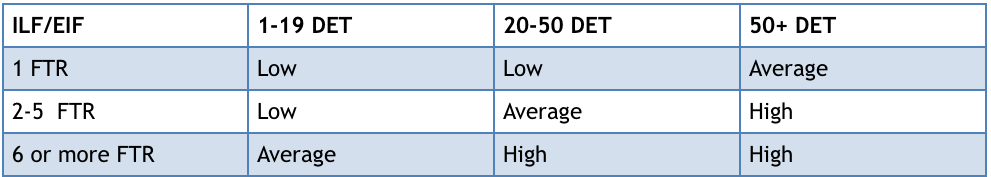
\includegraphics[scale=0.3]{s12}
\vspace{0.5cm}
 
\textbf{EOs and EQs}\\
\vspace{0.5cm}
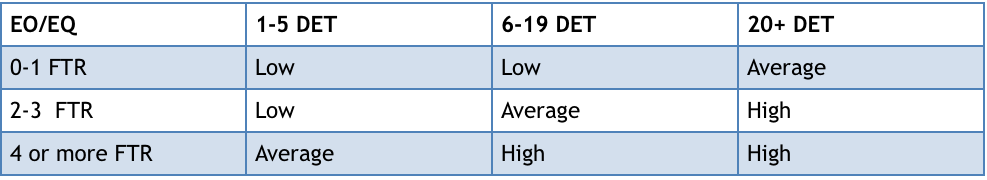
\includegraphics[scale=0.3]{s11}
\vspace{0.5cm}




\textbf{EIs}\\
\vspace{0.5cm}
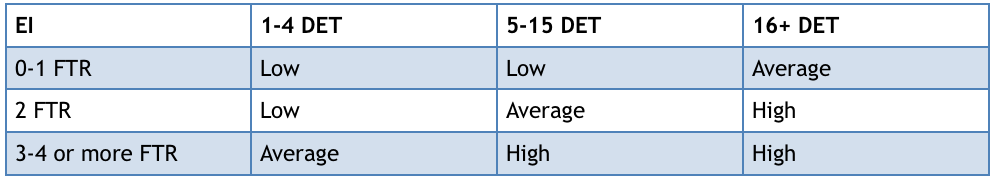
\includegraphics[scale=0.3]{s13}
\vspace{0.5cm}
\newpage
\textbf{UFP complexity weights}\\
\vspace{0.5cm}
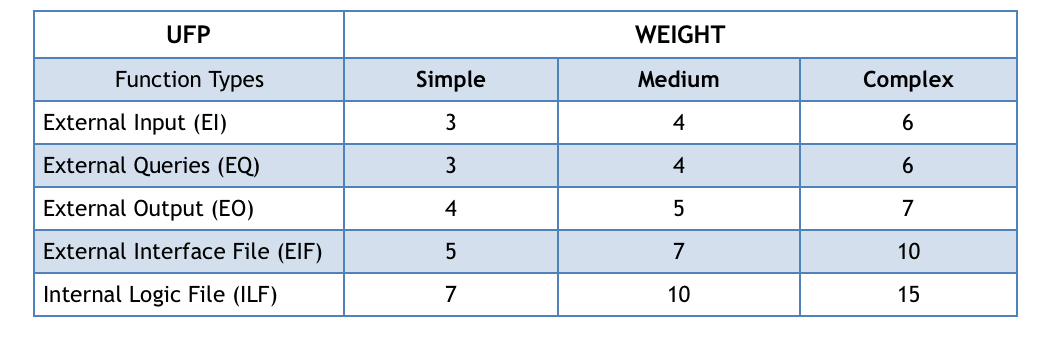
\includegraphics[scale=0.3]{s2}
\vspace{0.5cm}

\textbf{AFP complexity weights}\\
\vspace{0.5cm}
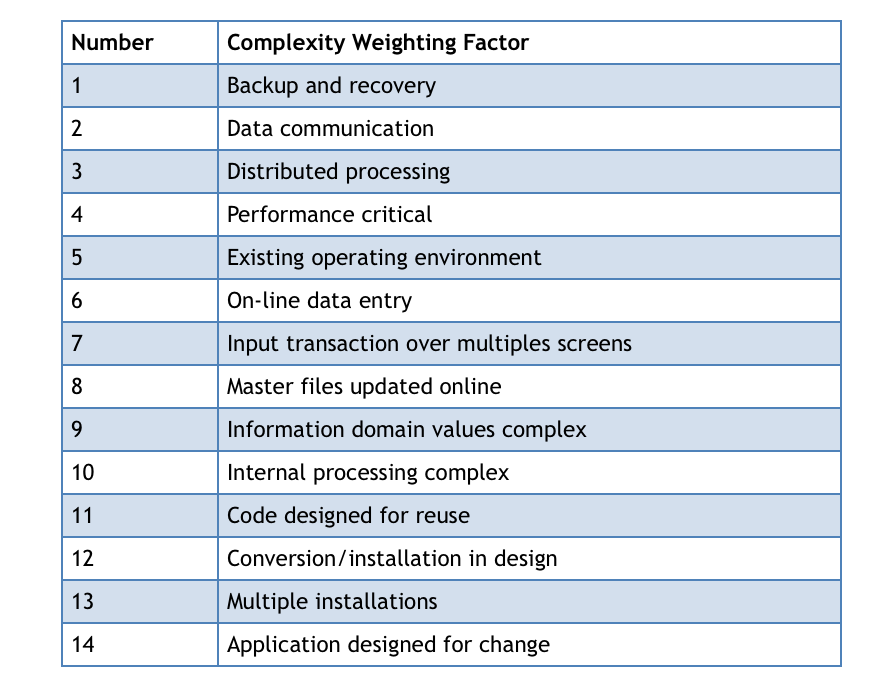
\includegraphics[scale=0.3]{s3}
\vspace{0.5cm}


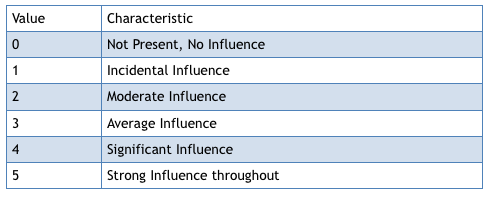
\includegraphics[scale=0.6]{s4}
\vspace{0.5cm}



\subsubsection{InternalLogicFiles(ILFs)}  %2.1.1 
In this paragraph we identify and analyse the IFls (i.e the internal logic files used by the application in order to store the data it needs to provide its functionalities) .\\
\vspace{0.5cm}
\textbf{User Data}
The application uses a single table to store  all the data about the users, that consist of \\
\begin{description}
\item\textbf{first name : String} 
\item \textbf{last name : String}     
\item \textbf{userId : String} 
\item \textbf{email : String} 
\item \textbf{password : String} 
\item \textbf{fiscal Code : String} 
\item \textbf{driving license code : String}
\item \textbf{credit card number code : String}
\item \textbf{birthday date : Date}
\end{description}

\vspace{0.5cm}

\textbf{Operator Data}
The application uses a single table to store all the data about the operators, that consist of:
\begin{description}
\item\textbf{first name : String} 
\item \textbf{last name : String}     
\item \textbf{operatorId : String} 
\item \textbf{email : String} 
\item \textbf{password : String} 
\item \textbf{fiscal Code : String} 
\item \textbf{driving license code : String}
\item \textbf{stationId: String}

\item \textbf{birthday date : Date}
\end{description}


\vspace{0.5cm}
\newpage
\textbf{Car Data}\break
The application uses a single table to store all the data about the electric cars.  The table contains the following set of attributes : \\

\vspace{0.5cm}


\begin{description}
\item\textbf{carId : String} 
\item \textbf{userId : String}     
\item \textbf{currentBattery : float} 
\item \textbf{latitude : float } 
\item \textbf{longitude : float} 
\item \textbf{issues : String} 
\item \textbf{in repair : Boolean}
\item \textbf{isAvailable: Boolean}

\end{description}
\vspace{0.5cm}








\textbf{Station Data} \break
The application uses a single table to store information about the stations: 
\vspace{0.5cm}


\begin{description}
\item \textbf{stationId : String} 
\item \textbf{ latitude : float}     
\item \textbf{ longitude : float} 
\item \textbf{ cars : int } 


\end{description}







\textbf{Reservation Data} \break
For the reservation data the application uses 2 different tables: one is used to store the ongoing reservations (i.e. those which have been done by users within an hour from the current time, and haven't been canceled), while the other table is used to store all past reservations, including the ones that have been cancelled. Both tables have the following set of attributes:\\
\begin{description}
\item \textbf{reservationId : String} 
\item \textbf{userId : String}     
\item \textbf{carId : String} 
\item \textbf{date : Date } 

\item \textbf{timer : Float } 
\item \textbf{isCancelled : Boolean } 

\end{description}


\vspace{0.5cm}



\textbf{Ride Data} \break

For the ride data the application uses 2 different tables: one is used to store the ongoing rides (i.e. those which have been started by users and haven't ended yet), while the other table is used to store all past rides.
 Both tables have the following set of attributes:\\
 \begin{description}
\item \textbf{rideId : String} 
\item \textbf{userId : String}     
\item \textbf{carId : String} 
\item \textbf{date : Date } 
\item \textbf{initialTime : Float } 
\item \textbf{finalTime : Float } 
\item \textbf{initialPosition : Float } 
\item \textbf{finalPosition: Float } 
\item \textbf{passengers : Int } 
\item \textbf{pitstops : Int } 
\item \textbf{isOnCharge : Boolean } 
\item \textbf{finalPrice : Float }
\item \textbf{pitstopTotalLength : float}  
\item \textbf{totalRideLength : Int } 
\item \textbf{lowCharge : Boolean } 
\item \textbf{accident: Boolean } 

\end{description}

Given the information above, w assign to each ILF the following scale factors. 

\vspace{0.5cm}

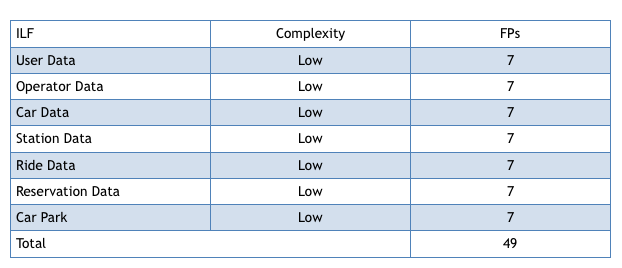
\includegraphics[scale=0.5]{ILF}


   






\subsubsection{External Logic Files (ELFs)} %2.1.2
The main external source of data of the application comes from the mapping service, which is mainly used to perform these operations:
\begin{itemize}
\item Given a starting and a final locations, compute the shortest path (as a  sequence of locations ) from the first location to the destination
\item Given an address, get the correspondent pair of coordinates (reverse geocoding)
\end{itemize}

On the client side, the mapping service is also used to retrieve the graphical representation of the city map to be displayed on the user's home page .\\

The following table  shows the assignments of the FPs values to each one of the ELF above:
\vspace{0.5cm}
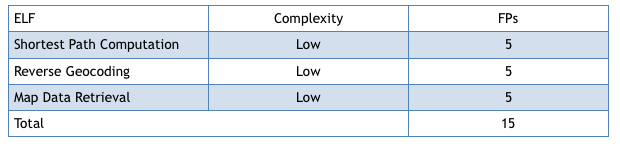
\includegraphics[scale=0.5]{ELF}




\subsubsection{External Inputs (EIs)} %2.1.3

The Power\&Joy application supports many kinds of interactions with users and operators.

\textbf{Users:}
\begin{itemize}
\item\textbf{Login/Logout (User)}these are simple operations, and count for 3FPs each
\item\textbf{Make reservation} This is a complex operation, so we are giving it 6 FPs
\item\textbf{Cancel reservation} This is a simple operation valuable of 3 FPs

\item\textbf{Start/End ride} Thse are complex operations, and require 6 FPs each
\item\textbf{Start/End PitStop} These are complex operations and require 4FPs each
\item\textbf{Report Accident} This is a complex operation, and requres 4FPs
\item\textbf{Assistance Needed} This is a simple operation, and involves only 3FPs
\item\textbf{Set User profile} This is a complex operation and rquires 4FPs
\item\textbf{Password retreival} This is a complex operation, and requires 4FPs
\item\textbf{View historical rides} This is a simple operation, and requires only 3FPs
\item\textbf{User Registration} This is a complex operation, and requires 4FPs

\end{itemize}

\textbf{Operators:}
\begin{itemize}
\item\textbf{operator Registration} This is a complex operation, and requires 4 FPs

\item\textbf{Login/Logout operator} These are simple operations, and require 3FPs each
\item\textbf{Operate}This is a complex operation, and require 6FPs
\item\textbf{Issue Solved} This is a quite complex operation, valuable for 4Fps
\item\textbf{Request Service Statistics}These operation involves complex queries, so it requires 6FPs
\end{itemize}

The following table assigns the FPs to each one of these functions:

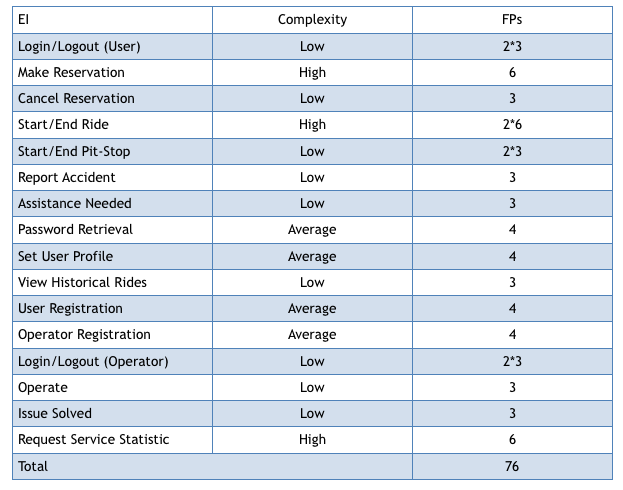
\includegraphics[scale=0.5]{EI}

\newpage
\subsubsection{External Inquiries (EQs)} %2.1.4
Since inquiries are just data requests from the users and operators, they can be seen as simple operations. The inquiries supported by our application are the following:\\
\vspace{0.5cm}
\textbf{Users:}

\begin{itemize}
\item Request cars to reserve
\item Retrieve reservation info
\item Retrieve ride info
\item Retrieve personal profile data
\item Retrieve reservation history
\end{itemize} 




\textbf{Operators:}
\begin{itemize}
\item Request the list of all cars 
\item request the list of issued cars
\item request the list of cars the are being repaired 
\item Retrieve reservation info
\item Retrieve ride info
\item Retrieve personal profile data
\item Retrieve reservation history
\end{itemize} 

The following table assigns the FPs to each one of these functions:

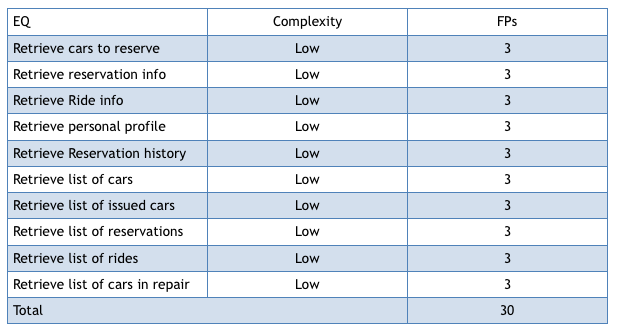
\includegraphics[scale=0.5]{EQ}


\subsubsection{External Outputs (EOs)} %2.1.5
Th Power\&Joy application sometimes needs to communicate with users and operators outside the contest of an enquiry, in order to accomplish the following functions:

\textbf{Users}
\begin{itemize}
\item Notify user that car has been reserved 
\item Notify user the cost of the ride when it end
\item Notify the user that he left the car 3km (or more) away from the nearest charging station (at the end of the ride)

\end{itemize}


\textbf{Operators}
\begin{itemize}
\item Notify the operator with the information (current position, issues, user, ecc. ) about the car he wants to take car of
\end{itemize}

Moreover, the system also needs to communicate with the external system that takes care of the payments for the rides. \\
The following table assigns the FPs to each one of these functions:

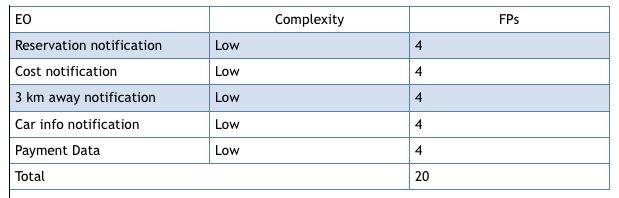
\includegraphics[scale=0.5]{EO}



\newpage
\subsubsection{Overall estimation} %2.1.6

Before going on with the final results, we are going to calculate the adjustment factors in order to compute the TDI (Total degree of influence) :

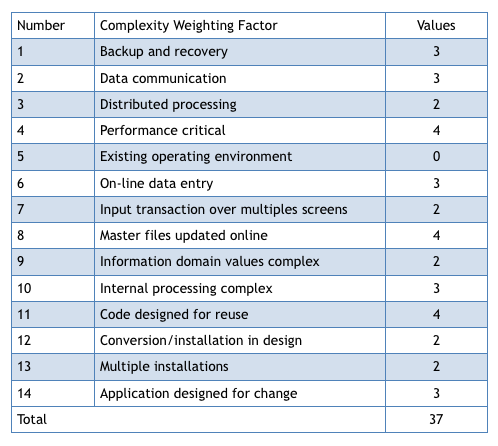
\includegraphics[scale=0.5]{AFP}

Thus we have 
\[TDI = 37\]
so that the VAF (Value adjustment factor) results
\[VAF = (TDI/100) +0.65 = (37 /100) + 0.65= 1.02 \]


The following table summarises the results of our EFP estimation activity:

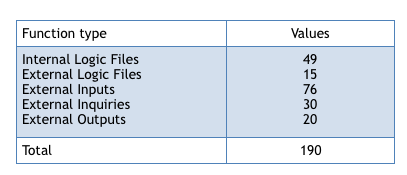
\includegraphics[scale=0.5]{FP} \\

Considering Java Enterprise Edition as a development platform and disregarding the aspects concerning the implementation of the mobile applications (which can be thought as pure presentation with no business logic), we can estimate the total number of lines of code.
Depending on the conversion rate, we have a lower bound of:

\[ UFP= 183 * 46 = 8418 \]


and an upper bound of

\[ UFP = 183 * 67 = 12261 \]

and the adjusted values are computed as 

\[SLOC= UFP * VAF \]

which gives as an upper bound 

\[ SLOC= 8418 * 1.02 =    8586      \]
 and as a lower bound
 
 \[SLOC = 12261 * 1.02 = 12506      \]


\subsection{Cost and effort estimation: COCOMO II} %2.2
In this section we're going to use the COCOMO II approach to estimate the cost and effort needed to develop the Power\&Joy system .



\subsubsection{Scale Drivers} %2.2.1
In order to evaluate the values of the scale drivers, we refer to the following o COCOMO II table
\vspace{0.5cm}
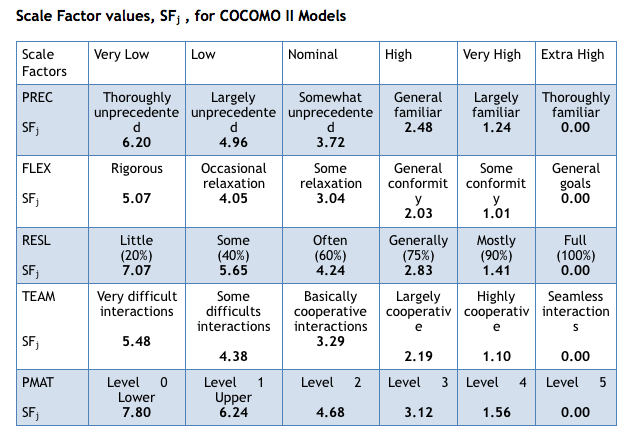
\includegraphics[scale=0.5]{cocomo/scale}
\vspace{0.5cm}
\newpage
Follows a short description for each driver:
\begin{description}
\item[Precedenteness] it's a parameter that describes the previous experience of our team with the development of large scale projects. Since we are not expert in the field, this value will be low.
\item[Development flexibility] it's a parameter that describes the degree of flexibility in the development process with respect to the external specification and requirements. Since there are very strict requirements on the functionalities but nothing specific is stated as for the technology to be used, this value will be low.
\item[Risk resolution] it's a parameter that describes the level of awareness and reactiveness with respect to risks. The risk analysis we performed is quite extensive, so the value will be set to  high.
\item[Team cohesion] it's a parameter that describes how well the team members know each other and work together in a cooperative way. For our team, the value is very high.
\item[Process maturity] it's a parameter that describes how well the goals have been achieved. Since we managed to achieve every goal, even if with some difficulties, this parameter will be medium valuated
\end{description}

These are the final results:
\vspace{0.5cm}
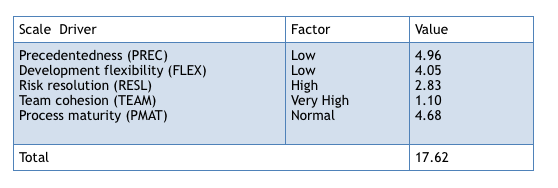
\includegraphics[scale=0.5]{cocomo/scaleValues}


\newpage
\subsubsection{Cost Drivers}%2.2.2
These are the cost drivers we are going to refer to in order to estimate the cost of the development of our application:

\begin{itemize}



\item Required Software Reliability:
Since the application is the only way to reserve and drive the electric cars, the RELY cost driver is set to high.\\
\vspace{0.5cm}
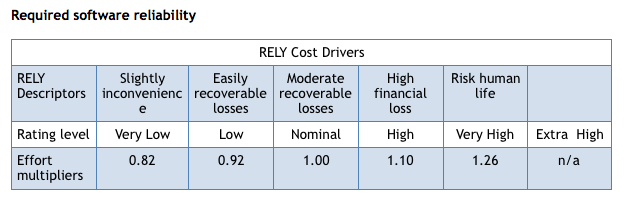
\includegraphics[scale=0.5]{cocomo/1_RELY}
\vspace{0.5cm}
\item Database size: 
Since the SLOC value is ranging between 8000 and 12000, we decided to place the DATA driver to normal .\\
\vspace{0.5cm}
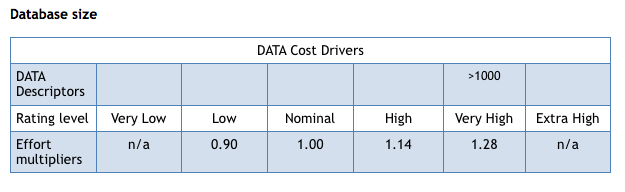
\includegraphics[scale=0.5]{cocomo/2_DATA}
\vspace{0.5cm}
\item Product complexity:  is set to high, given the results of the scale drivers .\\
\vspace{0.5cm}
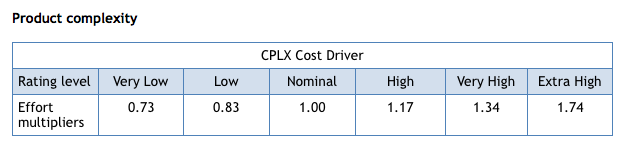
\includegraphics[scale=0.5]{cocomo/3_CPLX}
\vspace{0.5cm}
\item Required reusability: reusability is really important in our project, for further developments plans, so the RUSE driver is set to high.\\
\vspace{0.5cm}
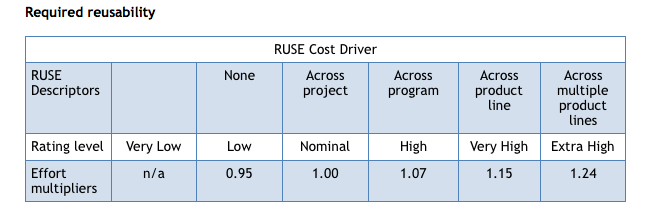
\includegraphics[scale=0.5]{cocomo/4_RUSE}
\vspace{0.5cm}
\item Documentation match to life-cycle needs: set to normal, since every aspect of our application has been analysed in  the documentation.\\
\vspace{0.5cm}
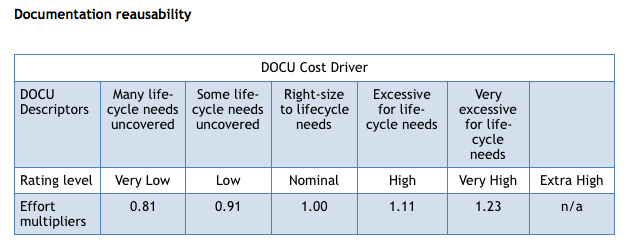
\includegraphics[scale=0.5]{cocomo/5_DOCU}

\item Execution time constraint: We expect the CPU usage is going to be very high, given the project complexity and the expected number of users.\\
\vspace{0.5cm}
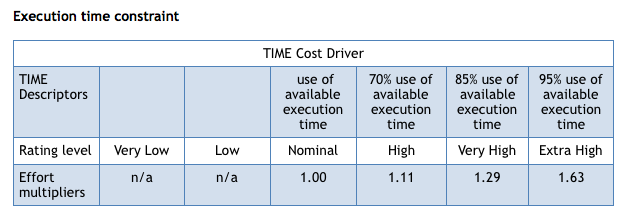
\includegraphics[scale=0.5]{cocomo/6_TIME}
\vspace{0.5cm}
\item Storage constraint: this parameter is set to normal, since we don't expect having problems of storage, given the currently available technologies. \\
\vspace{0.5cm}
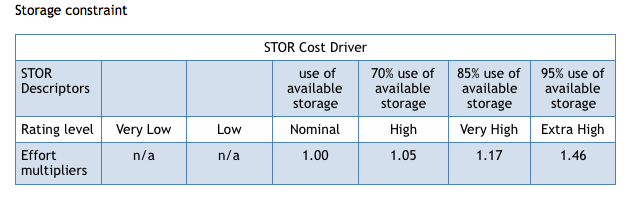
\includegraphics[scale=0.5]{cocomo/7_STOR}
\vspace{0.5cm}
\item Platform Volatility: this parameter is set to normal, since we don't expect to be doing major updates really often, except for the clients.\\
\vspace{0.5cm}
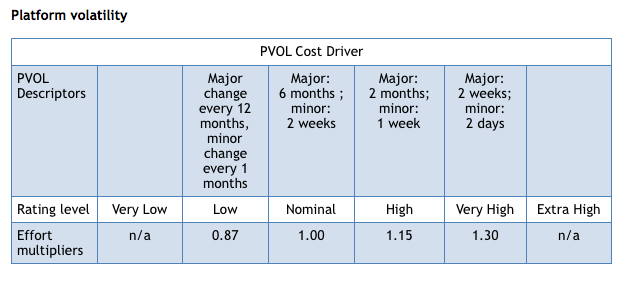
\includegraphics[scale=0.5]{cocomo/8_PVOL}
\item Analyst Capability: We think the analysis of the problem has been conducted in a thorough and complete way with respect to a potential real world
implementation. For this reason, this parameter is set to high.\\
\vspace{0.5cm}



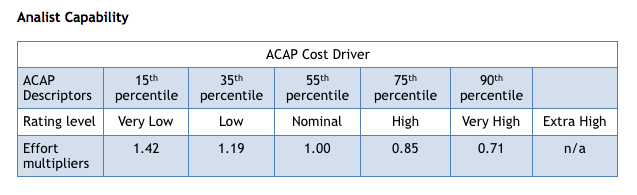
\includegraphics[scale=0.5]{cocomo/9_ACAP}
\vspace{0.5cm}
\item Programmer Capability: Set to normal, since we don't have that much of experience in project implementation yet.\\
\vspace{0.5cm}
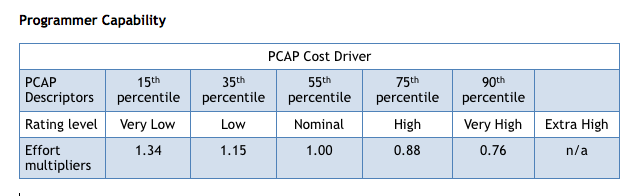
\includegraphics[scale=0.5]{cocomo/10_PCAP}
\vspace{0.5cm}
\item Application Experience: we have no much experience in the development of such large scale applications, so we set this driver to low.\\
\vspace{0.5cm}
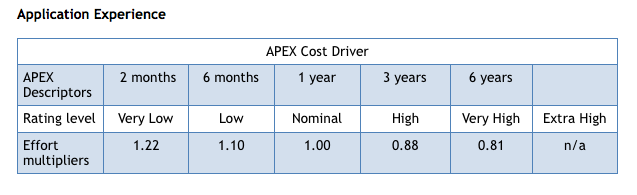
\includegraphics[scale=0.5]{cocomo/11_APEX}
\vspace{0.5cm}
\item Platform Experience: We don't have any experience with the Java EE platform, so this parameter is set to normal\\
\vspace{0.5cm}
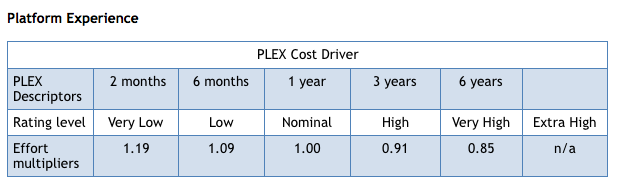
\includegraphics[scale=0.5]{cocomo/12_PLEX}
\vspace{0.5cm}
\item Language and Tool Experience: We don't have any experience with the Java EE platform, so this parameter is set to normal\\
\vspace{0.5cm}
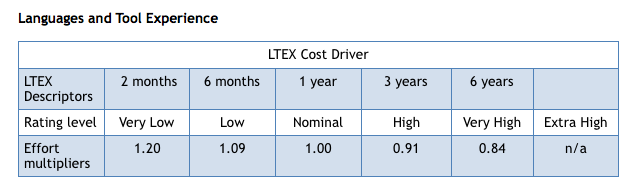
\includegraphics[scale=0.5]{cocomo/13_LTEX}
\vspace{0.5cm}
\item Personnel continuity: set to very low, since we don't have to actually develop the software\\
\vspace{0.5cm}
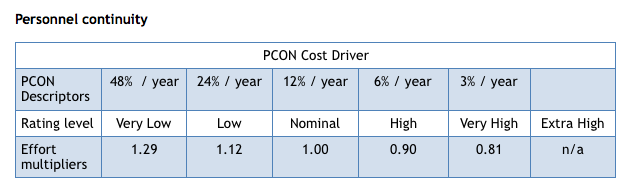
\includegraphics[scale=0.5]{cocomo/14_PCON}
\vspace{0.5cm}
\item Usage of Software Tools: Our application environment is complete and well integrated, so
we'll set this parameter to high.\\
 \vspace{0.5cm}
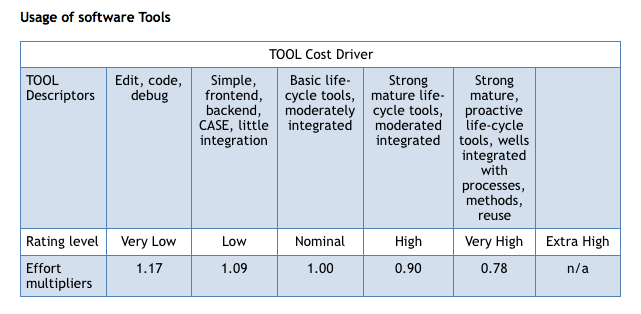
\includegraphics[scale=0.5]{cocomo/15_TOOL}
\newpage
\item Multisite development: we mostly communicated via Internet while working on this project, so we are going to set this parameter to high\\
\vspace{0.5cm}
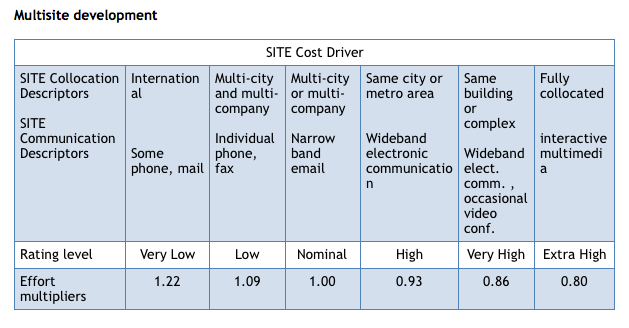
\includegraphics[scale=0.5]{cocomo/16_SITE}
\vspace{0.5cm}
\item Required development schedule: The definition of all the required documentation took a consistent amount of time, especially for the requirement analysis and the design stages. For this reason, this parameter is set to high.\\
\vspace{0.5cm}
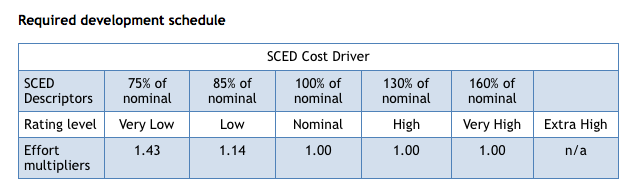
\includegraphics[scale=0.5]{cocomo/17_SCED}
\vspace{0.5cm}










\end{itemize}

\newpage
The following table reassumes the value assignments for each one of the fields described above:\\
\vspace{0.5cm}
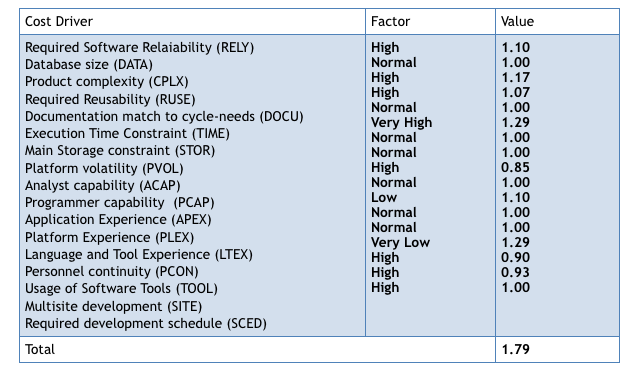
\includegraphics[scale=0.5]{cocomo/final}








\subsubsection{Effort equation}%2.2.3
This final equation gives us the effort estimation measured in Person-Months (PM):
 \[Effort = A * EAF * KSLOC^E    \]
 where:
 
 A = 2.94 (for COCOMO II)\\
EAF=product of all cost drivers (1.79)\\
E = exponent derived from the scale drivers. It is computed as:\\
\[E = B+ 0.01 * \sum {SF[i]} = B+ 0.01 * 17.62 = 0.91 + 0.1762 = 1.0862\]
 in which B is equal to: 0.91 for COCOMO II. 
 
 
 With this parameters we can compute the effort value, which has a lower bound of:
  \[Effort = A * EAF * KSLOC^E   = 2.94 * 1.79 * 8.586 ^ {1.0862}  = 54.39PM = 55PM\]
 
 and a lower bound of:
  \[Effort = A * EAF * KSLOC^E  = 2.94 * 1.79 * 12.506 ^ {1.0862}  = 81.82PM = 82PM \]
\newpage
\subsubsection{Schedule estimation}%2.2.4
As concerns the final schedule, we are going to use the following formula:
\[Duration = 3.67 * Effort^E\]

where F is computed as :
\[F = 0.28 + 0.2 * {E - B} = 0.28 + 0.2 * {1.0862 - 0.91} = 0.31524\]
having E = 1.0862 and B = 0.91 as seen above


Finally As a lower bound, we have Effort = 54.39 and
\[ Duration = 3.67 * 54.39^{0.31524} = 12.9351 months\]

and as an upper bound  we have Effort = 81.82 and
\[ Duration = 3.67 * 81.82^{0.31524} =14.712 months  \]

which both seem reasonable results.




\section{Schedule} %3
In this chapter we're going to provide an high-level project schedule. More refined schedules will be defined during the project to manage the internal organisation of the single development phases.
Notice that, even if this project is being for didactic purposes (such that no implementation and testing activities are going to be performed), we have considered these steps as part of our schedule as well. In order to take into account what could be the full development of this project.
\newpage
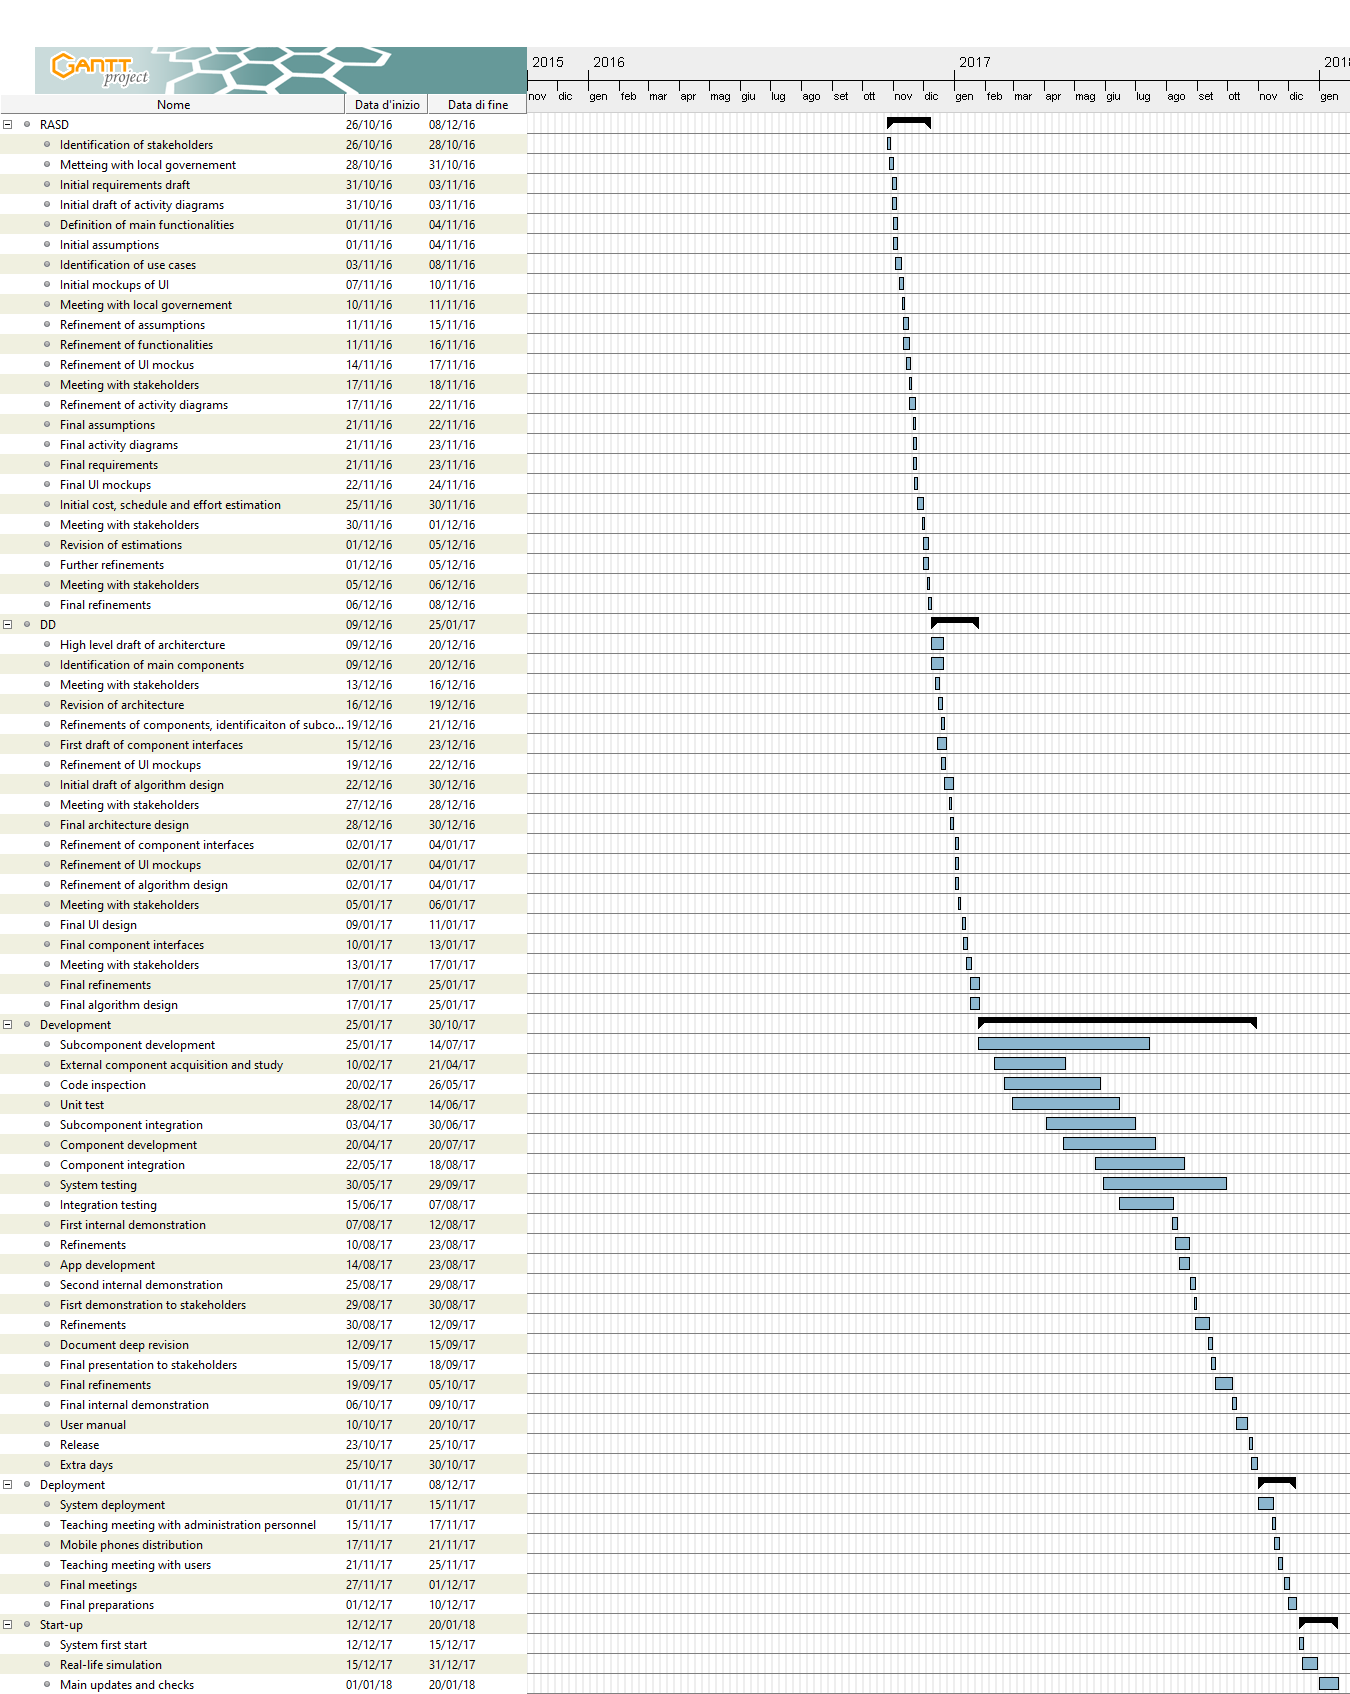
\includegraphics[scale=0.3]{gantt1}


\section{Resource Allocation} %4

In this chapter we're going to provide a general overview of how the tasks defined by the schedule in the previous section will be divided between the two members of our development team. More refined schedules will be defined during the project to manage the internal organisation of the single development phases.
As we already mentioned in the previous section, we have also included activities in the requirement analysis and design phases that won't actually take place, like the stakeholders meetings, as well as the full implementation phase. This has been purposefully done to have a more realistic depiction of how the development process could go. 
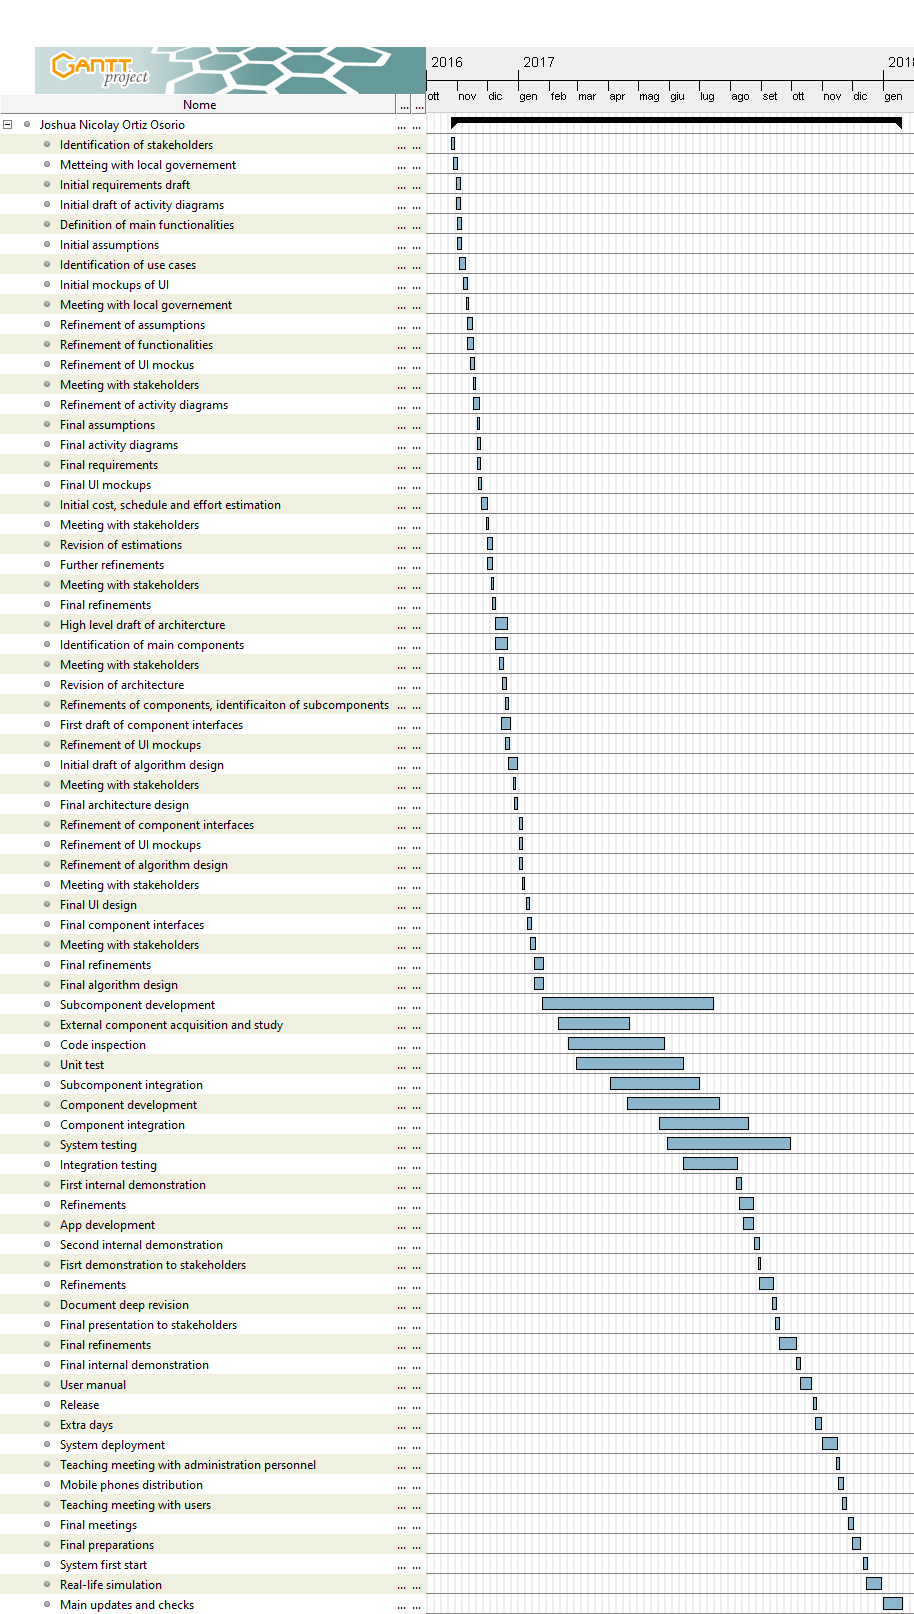
\includegraphics[scale=0.3]{ganttNico}
\newpage
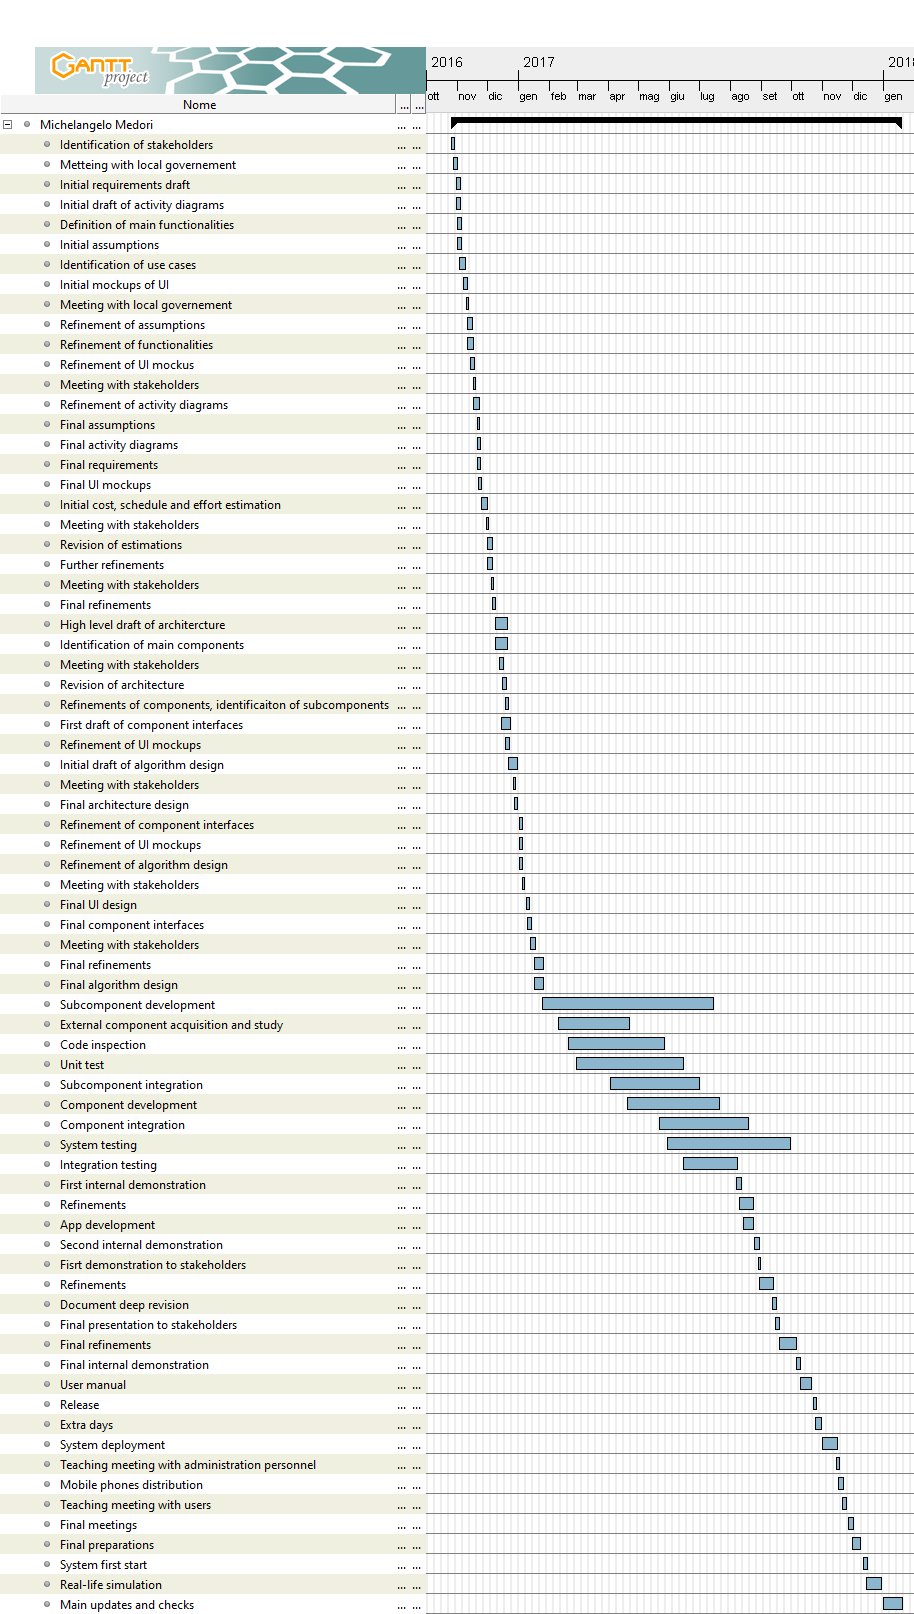
\includegraphics[scale=0.3]{ganttMike}
\newpage

\section{Risk Management } %5

In this section we are going to analyse the main risks that the project development may face. Some of them could derive from possible technical issues, while others come from political or financial dynamics .
First of all, a major threat is represented by our main political stakeholder, which is the city administration. Notice that up to now we have been  considering Milan's urban centre, but without focusing or relying much to Italy's laws, since we assumed that the system could be applied to any industrialised city, or even expand from a single city to an entire region or nation. Potential issues can include a change of the city government, a budget crisis (possibly as a secondary effect of some nationwide policy of spending review) or other shifts in the local government priorities. The main solution to this issue is to actively  involve the political stakeholders (i.e. at least  member of the city government ) in the requirement analysis and design stages, as well as the implementation one. Activities in this direction may include periodical reviews and meetings, demonstrations, discussions on the interface design and so on, with possible negotiations to be made.
Another related political issue concerns the possible changes in the national legislation. In particular, we are mainly concerned with modifications to the way car sharing  services are operated in general (for instance revisions of the driving license format or other restrictions), on the rules concerning electric cars (for example charges on the electric current or on the disposal of the charging stations) and to the possibility of using a smartphone while driving. There are already some limitations to this, but today they are overcome by avoiding to actively interact with the device and by keeping it fixed in a position that doesn?t interfere with the vision of the road. Stricter laws could be enacted in the future that forbid this possibility and require, for instance, that only voice interactions are allowed.   
Other issues might arise regarding the acceptance of the system from its intended users, both taxi drivers and passengers. As this system is going to completely replace the previous taxi management service, it is reasonable to assume that it?s going to face some initial opposition from people unwilling to change their habits (maybe because of the electric cars concept ). To make the transition easier, we suggest considering a few marketing strategies aimed at winning the support of the majority of the users. These can include acceptance tests, special offers and discounts for an initial period of time or other kinds of incentives.
We also have to consider issues arising from people management inside our company. Key members of the team may get ill just prior to important milestones or meetings, or may be ill for prolonged periods of time, causing delays. Also, we have to consider the possibility of people quitting the company, as the IT job market is quite flexible. A possible solution for this problem is to split duties and responsibilities across multiple people, so that no single person is in charge of a specific task.
Another risk might come from overestimating the knowledge of a specific matter or programming technique that our programmers and engineers have. Adding people to the project should not be seen as the primary solution here, unless the task is extremely specific. A good antidote is to hire knowledgable and flexible people beforehand.
Obviously, a loss of the whole source code, or significant parts of it , would be a disaster. This issues is quite easy to prevent, by implementing appropriate versioning systems and backup techniques distributed over multiple, redundant locations.
Another issue that must not be underestimated is related to our dependency on external services and components. A change in the terms and conditions of the Mapping Service, for example, could pose serious financial or technical problems. We are somewhat more protected as for database  as there is a greater number of vendors and the access methods are more or less standardised.
 Also, a change in the pricing plans of the cloud infrastructure could lead to significant issues on the financial and business side.
 A final problem may also emerge from issues with the project scheduling. Even though an initial overall schedule is provided in this document, it can?t obviously take into account all the possible issues that may arise down the road. For this reason, some extra time has been allocated at the expected end of each major activity to allow for adjustments.


\section{ChangeLog} %6
\begin{itemize}
\item Version 1.0 : initial version
\end{itemize}
\section{Hours of Work} %7

To redact this document, we spent 15 hours per person. We also report here the overall amount of hours per person required by the project.


 \end{flushleft}
\end{document}